В \textbf{первой главе} приведены основные понятия теории нечётких множеств и описаны актуальные модели представления нечёткой информации, используемые в дальнейшем при описании исследования. Дано определение нечётких моделей и их классификация в~зависимости от этапа применения нечёткой математики~--- при описании системы, при задании параметров, при задании входов, выходов и состояний (модели первого, второго и третьего типа). В работе предложена классификация нечётких моделей на основе применяемого в них языка описания выбора, объединённая с вышеописанной (рис.~\ref{fig:choice-classification}). В качестве объекта исследования выбраны модели, использующие чёткие отношения и нечёткие параметры (модели второго типа).
\begin{figure}[h] 
  \center
  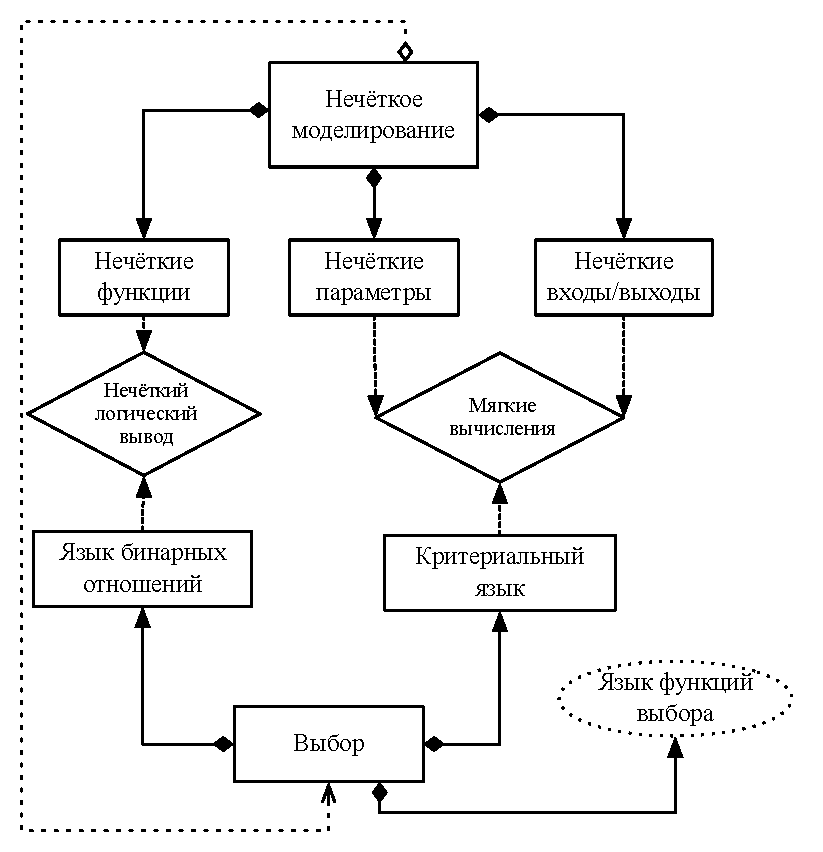
\includegraphics[scale=0.8]{choice-classification}
  \caption{Предлагаемая классификация нечётких моделей} 
  \label{fig:choice-classification}
\end{figure}

Особенностью рассматриваемых моделей является то, что существующие подходы к нечётким вычислениям далеко не всегда применимы в них. Нечёткий логический вывод неадекватен моделям второго типа, поскольку рассчитан на нечёткость отношений, отсутствие формализованных математических моделей либо способов решения с помощью классической теории. Лежащие в основании большинства способов <<мягких вычислений>> алгебраические структуры (в основном решётки) и отсутствие отношения линейного порядка приводят к нарушениям естественных математических отношений и неоправданному расширению неопределённости результата. В диссертации формулируются основные требования к модели представления нечёткой информации и методам решения задач второго типа~--- получение устойчивого решения, непротиворечивость естественным математическим отношениям, ограничение расширения неопределенности,~--- и вводятся требования вычислительной эффективности и возможности применения стандартных программных комплексов, предназначенных для чётких вычислений.

\textbf{Вторая глава} диссертации посвящена разработке и исследованию методов моделирования и обработки нечетких числовых величин, которые удовлетворяли бы выдвинутым к ним в главе 1 требованиям. Ввиду широкого распространения линейных моделей, исследование проводится для нечётких треугольных чисел. В качестве основной формы представления треугольных чисел в работе выбрана форма~\eqref{eq:membership-alphacut-form} в~виде границ чётких $\alpha$-интервалов $X_\alpha$, $\alpha \in \left[ 0;1 \right]$, позволяющая быстро переходить к интервальной неопределённости.
\begin{equation}
\label{eq:membership-alphacut-form}
	\left[ 
		\begin{aligned}
			& x^L(\alpha )=m-a+a\alpha  \\ 
			& x^R(\alpha )=m+b-b\alpha
		 \end{aligned}
	\right.
\end{equation}

Проводится краткий анализ существующих алгебраических методов обработки нечётких чисел, выделяются их достоинства и недостатки с точки зрения применимости в нечётких моделях второго типа. Для преодоления выделенных в главе 1 недостатков существующих методов нечётких вычислений предлагается следующий подход. Исходная задача $\tilde{Y}=f\left( \tilde{X}, \tilde A \right)$ с нечёткими числовыми параметрами и~переменными рассматривается как совокупность задач с интервальной неопределенностью
\begin{equation}
\label{eq:alpha-equivalence}
	\tilde{Y} = f\left( \tilde X, \tilde A \right)\to \bigcup\limits_{\alpha =0}^{1}{y_\alpha}=f\left( X_\alpha, A_\alpha \right)
\end{equation}
с последующим переходом к полной определённости на каждом $\alpha$-уровне, для чего на каждом $\alpha$-уровне внутри интервала $X_\alpha$ выбирается точка $\bar{x}\left( \alpha  \right)$. В диссертации предлагается выбирать значение $\bar{x}\left( \alpha  \right)$ с~помощью линейного параметрического преобразования $L$
\begin{equation}
  \label{eq:L-transform-base}
  \bar{x}\left( \alpha  \right)=L\left( X_\alpha \right)=\lambda x^L \left( \alpha  \right)+\left( 1-\lambda  \right) x^R \left( \alpha  \right).
\end{equation}

Для треугольных чисел $\bar{x}\left( \alpha  \right)$ является линейной функцией ввиду линейности $x^L\left( \alpha  \right)$ и $x^R\left( \alpha  \right)$. После решения чётких $\alpha $-уровневых задач полученные результаты $y\left( \alpha  \right)$ аппроксимируются нечётким числом $\tilde Y^{*}=\left\{ y(\alpha )\left| \mu_{\tilde Y}(y)=\alpha \right. \right\}$, которое называется \textit{модифицированным решением} задачи~\eqref{eq:alpha-equivalence}.

Предлагаемый подход в своей основе имеет декомпозицию нечётких чисел по~$\alpha$-уровням. C~точки~зрения алгебр нечётких чисел, решение задачи с~использованием декомпозиции представляет собой переход от использования <<полноценных>> нечётких чисел к~алгебрам для~чисел $LL/RR$-типа~--- функция принадлежности чисел такого типа является обратной к~функции, которая определяет точки $\bar{x}\left(\alpha \right)$:
\begin{equation}
\label{eq:modified-inverse-function}
  \mu_{\tilde A^{*}}\left( x \right)={\left( \bar{x}\left( \alpha  \right) \right)}^{-1}
\end{equation}

В диссертации вводится ключевое понятие модифицированного нечёткого числа. \textit{Модифицированным нечётким числом} называется число $\tilde A^{*}$, получаемое из~$\tilde{A}$ с~помощью преобразования~\eqref{eq:L-transform-base} и~\eqref{eq:modified-inverse-function}. В работе показано, что модифицированное нечёткое число является числом $LL/RR$-типа, и в дальнейшем для таких чисел используется обозначение $\bar{x}\left( \alpha  \right)$, указывающее на механизм их построения с помощью~\eqref{eq:modified-inverse-function}.

Исходя из~\eqref{eq:L-transform-base} и~\eqref{eq:modified-inverse-function} очевидно, что преобразование~$L$ сокращает информативность исходной нечёткой величины. Для определения степени потери нечёткой информации исследуются свойства преобразования $L$. Чтобы производить анализ и~вычисления в~форме, нечувствительной к~знаку нечёткого числа, в диссертации предложено представление треугольного числа в виде тройки следующих параметров:
\begin{itemize}
  \item длина носителя $d_{\tilde A}$;
  \item мода $m_{\tilde A}$;
  \item степень асимметрии $AS_{\tilde A}$.
\end{itemize}

\textit{Степенью асимметрии} $AS_{\tilde A}$ называют характеристику треугольного нечёткого числа, определяемую как разность площадей прямоугольных треугольников, на которые исходное нечёткое число делится модой.

В работе показано, что~запись треугольного нечёткого числа в~виде тройки $\left(m_{\tilde A}, d_{\tilde A}, AS_{\tilde A} \right)$ эквивалентна введённым ранее способам записи через коэффициенты нечёткости $\left( m;a;b \right)$ и~точки пересечения с~осью $Ox$ $\left( x^L;m;x^R \right)$. При~известных степени асимметрии~$AS_{\tilde A}$ и~длине носителя~$d_{\tilde A}$, коэффициенты нечёткости определяются по~формуле
\begin{equation*}
	\left[ \begin{aligned}
      & a=\frac{d_{\tilde A}-2AS_{\tilde A}}{2} \\ 
      & b=\frac{d_{\tilde A}+2AS_{\tilde A}}{2} \\ 
    \end{aligned} \right.
\end{equation*}

Для преобразования $L$ доказаны следующие свойства, подтверждающие, что~его применение к~нечетким исходным данным в~основном сохраняет их~информативность при~целенаправленном выборе параметра $\lambda$, а уменьшение длины носителя можно рассматривать как~положительное явление, позволяющее снизить степень неопределённости решения.

\begin{prop}
\label{prop:L-prop1}
Преобразование $L$ сохраняет моду нечёткого числа. Другими словами, $\forall \lambda \in \left[ 0;1 \right]:\ m_{\tilde A}=m_{\tilde A^{*}}$.
\end{prop}

\begin{prop}
\label{prop:L-prop2}
При некоторых значениях параметра $\lambda$ преобразование $L$ сохраняет
\begin{enumerate}
  \item знак степени асимметрии, т.е. $\exists \lambda \in [0;1]:\ sign(AS_{\tilde A})=sign(AS_{\tilde A^{*}})$;
  \item значение степени асимметрии, т.е. $\exists \lambda \in [0;1]:\ AS_{\tilde A}=AS_{\tilde A^{*}}$.
\end{enumerate}
\end{prop}

\begin{prop}
\label{prop:L-prop3}
Модифицированное число всегда содержится внутри исходного числа. Другими словами, $\forall \lambda \in \left[ 0;1 \right]: A_{\alpha}^{*}\subset A_\alpha;\ d_{\tilde A} \geqslant d_{\tilde A^{*}}$, т.\,е. преобразование~$L$ уменьшает длину носителя нечёткого числа и~оставляет $\alpha$-интервалы модифицированного числа в~рамках $\alpha$-интервалов исходного числа.
\end{prop}

На основании следствий из свойств преобразования $L$, в диссертации даются рекомендации по выбору параметра $\lambda$ и применимости предлагаемой методики:
\begin{itemize}
  \item при $\displaystyle \lambda =\frac{a}{a+b}=\frac{a}{d_{\tilde A}}$ сохраняется значение степени асимметрии. Применение преобразования $L$ с этим значением $\lambda$ к нечётким $LL/RR$-числам не изменяет их;
  \item при $\displaystyle \lambda =\frac{b}{a+b}=\frac{b}{d_{\tilde A}}$ преобразование~$L$ уничтожает нечёткую информацию, заложенную экспертом в число, и сводит операции над числами к операциям над их модами;
  \item применимость преобразования $L$ при использовании симметричных нечётких числах ограничена, поскольку $\displaystyle \lambda =\frac{a}{a+b}=\frac{b}{a+b}=\frac{1}{2}$, и все вычисления в этом случае сводятся к операциям над модами чисел. 
\end{itemize}

Для доказательства применимости предложенного подхода в нечётких моделях второго типа, создаётся алгебраическая система для множества всех нечётких модифицированных чисел $K=\left\{ \bar{x}\left( \alpha  \right) \right\};\ \alpha \in \left[ 0;1 \right]$. Строится чёткая алгебра $P=\left\langle K ;\ +,\,* \right\rangle$ и показывается, что $Р$ удовлетворяем всем аксиомам поля. Для построения алгебры используется более удобная форма записи модифицированного числа
\begin{equation}
\label{eq:modified-number-base}
  \bar{x}\left( \alpha  \right)=c+k\alpha,
\end{equation}
где
\begin{equation}
\label{eq:modified-number-from-abm}
  \begin{aligned}
    & \left[ \begin{aligned}
    & c=m+b-\lambda \left( a+b \right) \\ 
    & k=\lambda \left( a+b \right)-b \\ 
  \end{aligned} \right. \\ 
  & \lambda \in \left[ 0;1 \right];\ c,k\in \mathbb{R} \\ 
\end{aligned}
\end{equation}

На~множестве $K$ вводится операция сложения~\eqref{eq:fuzzy-addition}, а также нейтральный~\eqref{eq:fuzzy-zero} и противоположный по сложению~\eqref{eq:fuzzy-minus} элементы. Доказываются свойства ассоциативности и коммутативности операции~\eqref{eq:fuzzy-addition}.
\begin{gather}
  \label{eq:fuzzy-addition}
  \bar{x}_1\left(\alpha \right)+\bar{x}_2\left(\alpha \right)=r_1\left( \alpha  \right)=c_1+c_2+\left(k_1+k_2 \right)\alpha,\ r_1 \left( \alpha  \right)\in K;\\
  \label{eq:fuzzy-zero}
  \bar{0}=0+0\alpha \in K: \forall \bar{x}(\alpha )\in K:\ \bar{x}(\alpha )+\bar{0}=c+k\alpha +0+0\alpha =\bar{x}(\alpha );\\
  \label{eq:fuzzy-minus}
  -\bar{x}\left(\alpha \right)=-c-k\alpha \in K:\ \bar{x}\left( \alpha  \right)+\left( -\bar{x}\left( \alpha  \right) \right)=\bar{0}. 
\end{gather}

Также на множестве $K$ вводится операция умножения. Её можно было бы определить с помощью~\eqref{eq:fuzzy-invalid-multiplication} как сумму произведений компонент модифицированных нечётких чисел
\begin{equation}
\label{eq:fuzzy-invalid-multiplication}
  \bar{x}_1(\alpha )\cdot \bar{x}_2(\alpha )=r_{2}^{'}\left( \alpha  \right)=\left( c_1+k_1\alpha  \right)\left( c_2+k_2\alpha \right)= c_1 c_2+c_1 k_2\alpha+c_2 k_1\alpha+k_1 k_2\alpha^2,
\end{equation}
однако такое определение приводит к искажению треугольного вида результата нечётких операций, т.е.~$r_{2}^{'}\left( \alpha  \right)\notin K$. Для того, чтобы результат операции умножения остался в~множестве~$K$, используется линейная интерполяция~--- зависимость $r_2\left(\alpha \right)$ восстанавливается в~виде линейной функции по значениям выражения~\eqref{eq:fuzzy-invalid-multiplication} при~$\alpha =0$ и~$\alpha=1$. Это приводит к следующему определению операции умножения:
\begin{equation}
\label{eq:fuzzy-multiplication}
  r_2\left( \alpha \right)=c_1 c_2+\left(c_1 k_2+ c_2 k_1 +k_1 k_2 \right)\alpha;\ r_2\left( \alpha  \right)\in K.
\end{equation}

Для операции умножения~\eqref{eq:fuzzy-multiplication} вводятся нейтральный~\eqref{eq:fuzzy-one} и обратный по умножению~\eqref{eq:fuzzy-division} элементы. Доказываются свойства ассоциативности и коммутативности, а также свойство дистрибутивности умножения~\eqref{eq:fuzzy-multiplication} относительно сложения~\eqref{eq:fuzzy-addition}. Показано, что для существования обратного элемента число $\bar{x}\left( \alpha  \right)$ должно иметь ненулевую моду, поскольку, согласно~\eqref{eq:modified-number-from-abm}, $c+k=m\ne 0$.
\begin{gather}
  \label{eq:fuzzy-one}
  \bar{1}=1+0\alpha \in K:\ \forall \bar{x}\left( \alpha  \right)\in K\quad \bar{x}\left( \alpha  \right)\cdot \bar{1}=\bar{x}\left( \alpha  \right); \\
  \label{eq:fuzzy-division}
  \bar{x}^{-1}(\alpha )=\frac{1}{c}-\frac{k}{c\left(c+k\right)}\alpha,\ c\ne 0;\ \bar{x}^{-1}(\alpha ) \in K:\ \bar{x}\left(\alpha \right){{\bar{x}}^{-1}}\left( \alpha  \right)=\bar{1}.
\end{gather}

В диссертации для модифицированных нечётких чисел показывается эквивалентность записи в~виде~\eqref{eq:modified-number-base} и в~виде
\begin{equation}
\label{eq:isomorphic-field}
  \bar{x}_{\tilde A}\left( \alpha \right)=\bar{x}_{\tilde A}\left( 0 \right)+\alpha \left(\bar{x}_{\tilde A}\left( 1 \right)-\bar{x}_{\tilde A}\left(0 \right) \right)=\alpha \bar{x}_{\tilde A}\left( 1 \right)+\left( 1-\alpha  \right) \bar{x}_{\tilde A}\left( 0 \right).
\end{equation}

На основании~\eqref{eq:isomorphic-field} предложен способ нечётких вычислений, называемый двухточечными вычислениями, позволяющий решать нечёткую задачу как две чёткие при $\alpha=0$ и $\alpha=1$. Если обозначить за~$*$ произвольную арифметическую операцию, то для~чисел в~форме~\eqref{eq:isomorphic-field} её результат будет выглядеть следующим образом:
\begin{equation}
\label{eq:two-point-calculations}
  \bar{x}_{\tilde A}\left( \alpha \right)*\bar{x}_{\tilde B}\left(\alpha \right)=\alpha \left(\bar{x}_{\tilde A}\left( 1 \right)*\bar{x}_{\tilde B}\left(1 \right) \right)+\left(1-\alpha \right)\left(\bar{x}_{\tilde A}\left(0 \right)*\bar{x}_{\tilde B}\left(0 \right) \right).
\end{equation}

В работе показано, что двухточечные вычисления сводятся к алгебре модифицированных нечётких чисел, избавляют от необходимости вводить отношение линейного порядка на множестве $K$ и~позволяют использовать стандартные программные продукты для решения нечетких задач, т.\,к. нечеткая задача решается как две чётких.

В качестве альтернативы вышеописанному методу решения задач в тех случаях, когда потери экспертной информации недопустимы, предлагается использовать двухкопмонентные нечёткие числа. Данный подход позволяет свести операции над нечёткими треугольными числами к операциям над их левой и правой частями, т.\,е. к ранее описанной алгебре модифицированных нечётких чисел $LL/RR$-типа.

В конце второй главы кратко рассматривается проблема устойчивости моделей второго типа на примере задачи линейного программирования с нечёткими параметрами
\begin{equation*}
  \left\{ \begin{aligned}
    & f\left( \mathbf{x} \right)=\mathbf{Cx}\to \min;  \\ 
    & \mathbf{Ax}=\mathbf{B},
  \end{aligned} \right.
\end{equation*}
где $\mathbf{A}=\left\{ \tilde{A}_{ij} \right\}$~--- матрица, а~$\mathbf{B}=\left\{ \tilde{B}_i \right\}$, $\mathbf{C}=\left\{\tilde{C}_i \right\}$~--- векторы нечётких параметров. 
Применение к~каждому из~элементов матрицы и~векторов преобразования~$L$ приводит к модифицированной задаче
\begin{equation}
\label{eq:fuzzy-lp-unstable-problem}
  \left\{ \begin{aligned}
    & f\left( \mathbf{x} \right)={\mathbf{C}^{*}}\mathbf{x}\to \min;  \\ 
    & {\mathbf{A}^{*}}\mathbf{x}={\mathbf{B}}^{*},
  \end{aligned} \right.
\end{equation}
в~которой $\mathbf{A}^{*}=\left\{ \bar{x}_{\tilde{A}_{ij}}\left(\alpha \right) \right\}$, $\mathbf{B}^{*}=\left\{ \bar{x}_{\tilde{B}_i}\left(\alpha \right) \right\}$, $\mathbf{C}^{*}=\left\{ \bar{x}_{\tilde{C}_i}\left(\alpha \right) \right\}$.

При~изменении значений $\alpha$ при~фиксированных коэффициентах $\lambda_{A_i}$ преобразования~$L$, происходит~возмущение задачи~\eqref{eq:fuzzy-lp-unstable-problem}. Ввиду свойства сохранения моды, в работе предлагается зафиксировать в~качестве <<эталонного>> решение~\eqref{eq:fuzzy-lp-unstable-problem} при~$\alpha=1$ и использовать определение устойчивости по~решению, поскольку оно включает в~себя более узкое определение общей устойчивости, т.\,е. принципиальное существование решения возмущённой задачи. Предполагается, что нечёткая задача будет считаться устойчивой по решению, если при переходе с одного $\alpha$-уровня на другой не происходит значительного изменения решения относительно $\mathbf{x}\left( \alpha =1 \right)$, т.\,е.
\begin{equation}
\label{eq:fuzzy-solution-stability}
  \forall \varepsilon >0\ \exists \delta >0:\forall \alpha \in \left[0; 1\right)\ \left| \alpha -1 \right|<\delta \Rightarrow \left\| \mathbf{x}\left( 1 \right)-\mathbf{x}\left( \alpha  \right) \right\|<\varepsilon.
\end{equation}

Согласно методике двухточечных вычислений, задачу~\eqref{eq:fuzzy-lp-unstable-problem} достаточно решить на двух $\alpha$-уровнях. Получаемая пара векторов $\mathbf{x}\left( \alpha =1 \right)$ и $\mathbf{x}\left( \alpha =0 \right)$ позволяет восстановить модифицированные решения согласно~\eqref{eq:isomorphic-field}. Ввиду свойства сохранения моды, решение модифицированной задачи~\eqref{eq:fuzzy-lp-unstable-problem} при $\alpha=1$ аналогично решению чёткой задачи с~коэффициентами, равными модам нечётких чисел. Если решать ту~же задачу при~$\alpha=0$ без дополнительных ограничений на~параметры $\lambda_S$ преобразования $L$, то~возникает ситуация, при~которой все~значения $\lambda_S$, где~$S$~--- один из индексов $\tilde A_{ij}$, $\tilde B_i$, $\tilde C_i$,~--- принимают единичные значения. Это объясняется тем фактом, что при $\lambda_S=1$ максимальный вес в значении $\bar{x}_S\left(\alpha \right)$ имеет левая ветвь функции принадлежности, находящаяся ближе к нулю. Для решения данной проблемы вводятся дополнительные ограничения для параметров $\lambda_S$:
\begin{equation}
\label{eq:lambda-minimization-criterion}
  {\left( \lambda_{S}^{\star}-\lambda_S \right)}^2\to \min
\end{equation}
которые позволяют минимизировать отклонение параметров от оптимальных в~смысле сохранения нечёткой информации значений $\displaystyle \lambda_{S}^{\star}=\frac{a_S}{d_S}$ и, таким~образом, управлять устойчивостью решения. Ввиду противоречивости критериев~\eqref{eq:lambda-minimization-criterion} и~целевой~функции задачи~\eqref{eq:fuzzy-lp-unstable-problem}, возникает задача векторной оптимизации, для решения которой используется аддитивная свёртка критериев:
\begin{equation}
\label{eq:modified-target-function}
  f^{*}\left( \mathbf{x} \right)=\mathbf{C}^{*}\mathbf{x}+\gamma \sum\limits_{s}^{}{\left(\lambda_{S}^{*}-\lambda_S \right)}^{2} \to \min
\end{equation}
Семантика целевой функции~\eqref{eq:modified-target-function} такова: ищется решение $\mathbf{x}$ и вектор параметров $\mathbf{\lambda}_S$ преобразования $L$, которые позволяют удовлетворить исходный критерий оптимизации и~при~этом максимально сохранить нечёткую информацию, заложенную экспертами в параметры задачи. Безразмерный коэффициент~$\gamma$ позволяет привести значение свёртки к~одному~порядку со~значением исходной целевой функции.

В \textbf{третьей главе} происходит тестирование разработанных моделей и методов обработки нечетких числовых величин на примере задачи сетевого планирования с нечёткими временными оценками. Кратко рассматривается классическая постановка задачи, связанные с ней определения и основные способы её решения, а также исследуются достоинства и недостатки существующих способов решения задачи сетевого планирования с нечёткими параметрами.

В качестве модели проекта в сетевом планировании рассматривается направленный ациклический граф $G=(V,E)$, $\left| V \right|=n$, $\left| E \right|=m$, в котором работам проекта $w_j$, длительностью $\tau_j$ каждая, сопоставлены дуги графа $e_j$, $j=\overline{1,m}$, а событиям проекта $z_i$ с~временами наступления $t_i$ сопоставления вершины графа $v_i$, $i=\overline{1,n}$. Событие $z_1$~--- начало работ по проекту, событие $z_n$~--- окончание проекта. Граф $G$ обладает следующими свойствами:
\begin{itemize}
  \item существует ровно одна вершина $v_1\in V$, называемая истоком, из которой рёбра только исходят, т.е. $\forall i=2,n$ $\nexists \left( v_i, v_1 \right)$;
  \item существует ровно одна вершина $v_n\in V$, называемая стоком, в которую рёбра графа только входят, т.е.  $\forall i=\overline{1,n-1}$ $\nexists \left( v_n, v_i \right)$;
  \item для любой вершины графа $v_i\in V,\ i=\overline{1,n}$ существует путь $v_1\ldots v_n$, проходящий через неё;
  \item для любого ребра $e_j\in E,\ j=\overline{1,m}$ существует путь $v_1\ldots v_n$, содержащий это ребро.
\end{itemize}

Задача сетевого планирования сводится к~поиску общего времени выполнения проекта $T$, которое равно длине максимального пути в графе, называемого также критическим. Соответственно, операции, которые принадлежат пути максимальной длины, также называются критическими. В диссертации указано, что алгоритмический метод решения задачи сетевого планирования (модифицированные алгоритмы Дейкстры и Форда-Мура-Беллмана) не позволяет проводить её анализ на устойчивость, т.е. на изменение критического пути. В качестве основного способа решения выбрано решение задачи линейного программирования~\eqref{eq:crisp-lp-cpm-task} с~нечёткими временными оценками
\begin{equation}
\label{eq:crisp-lp-cpm-task}
  T=t_n-t_1 \to \min
\end{equation}
при ограничениях на времена наступления событий
\begin{equation}
\label{eq:crisp-lp-cpm-restrictions}
  t_{j_s}-t_{i_s}\geqslant \tilde \tau_s;\ s=\overline{1,m},
\end{equation}
где $t_{i_s}$ и $t_{j_s}$~--- времена наступления событий начала и окончания работы $w_s$ соответственно. В~результате решения данной задачи получается общее время выполнения проекта $\tilde T$, а также вектор времён $\mathbf{t}=\left\{\tilde t_1, \ldots, \tilde t_n \right\}$, называемых календарным планом проекта, и~совокупность критических операций $\mathbf{S}_1$.

Для~решения задачи~\eqref{eq:crisp-lp-cpm-task}--\eqref{eq:crisp-lp-cpm-restrictions}, в работе применяется преобразование $L$ и~методика двухточечных вычислений. Формулируется задача для~произвольного $\alpha$-уровня
\begin{equation}
\label{eq:modified-fcpm-lp}
  \left\{ \begin{aligned}
    & T(\alpha )=t_n-t_1\to \min  \\ 
    & t_{j_s}-t_{i_s}\geqslant \bar{\tau}_s\left(\alpha,\lambda_s \right),\ \forall s=\overline{1,m}.
  \end{aligned} \right.
\end{equation}

Преобразование $L$, применяемое в~\eqref{eq:modified-fcpm-lp}, несколько отличается от вводимого формулой~\eqref{eq:L-transform-base}, поскольку параметры $\lambda$ необходимо изменять, управляя, таким образом, устойчивостью задачи линейного программирования. Результатом решения задачи~\eqref{eq:modified-fcpm-lp} является вектор времён $t\left( \alpha \right)=\left\{ t_0\left(\alpha\right),\ldots,t_n\left(\alpha \right) \right\}$, который является календарным планом $\alpha$-уровня, а~также множество критических операций $S_1\left( \alpha \right)$.

Нечеткость оценок $\tilde{\tau}_i$ обуславливает проблему устойчивости решений задачи~\eqref{eq:modified-fcpm-lp} в~смысле~\eqref{eq:fuzzy-solution-stability}. Для неустойчивой задачи на различных $\alpha$-уровнях решения соответствуют различным критическим путям, и~возникает проблема объединения разнородных $\alpha$-уровневых решений $S_1\left(\alpha \right)$. Согласно данному ранее определению~\eqref{eq:fuzzy-solution-stability}, задача~\eqref{eq:modified-fcpm-lp} поиска критического пути на $\alpha$-уровне считается устойчивой по~решению, если она устойчива и если $S_1$ не~зависит от $\alpha$, т.\,е. на всех $\alpha$-уровнях критический путь не изменяется и~проходит по~одним и~тем~же рёбрам. Отмечается, что условие устойчивости выполняется автоматически, поскольку в~сетевом графике всегда существует хотя бы один путь от истока к стоку, следовательно, независимо от величин весов рёбер, всегда существует путь максимальной длины. В~качестве метрики сходства решений в работе выбрана мощность симметрической разности двух множеств:
\begin{equation}
\label{eq:modified-cpm-lp-stability}
  \forall \alpha_1, \alpha_2\in \left[ 0;1 \right];\ \alpha_1\ne \alpha_2\ S_1\left(\alpha_1 \right)\Delta S_2\left(\alpha_2 \right)=\varnothing,
\end{equation}
т.\,е. на всех $\alpha $-уровнях критический путь не~изменяется и~проходит по~одним и~тем~же дугам. 

Полученное при $\alpha=1$ решение задачи~\eqref{eq:modified-fcpm-lp} даёт активные ограничения на критические операции. В диссертации отмечается, что на параметры $\lambda_S$ преобразования $L$ также необходимо наложить ограничения и учесть их в целевой функции~\eqref{eq:modified-target-function}, чтобы избежать ситуации, когда $\lambda_S$ принимают граничные значения (0 или 1). В~результате при $\alpha=0$ решается видоизменённая задача
\begin{equation}
\label{eq:modified-fcpm-lp-alpha}
  \left \{ \begin{aligned}
    & T^* \left(\alpha, \lambda \right) = t_n-t_1+\gamma \sum \limits_{s=1}^{m} \left(\lambda_s^*-\lambda_s \right)^2 \to \min; \\
    & t_{j_{s_1}}-t_{i_{s_1}} = \bar{\tau}_{s_1}\left(\alpha, \lambda_{s_1} \right),\ \forall s_1 \in S_1\left(1\right); \\
    & t_{j_s}-t_{i_s} \geqslant \bar{\tau}_s\left(\alpha, \lambda_s \right),\ \forall s \notin S_1\left(1\right),\,s=\overline{1,m}.
  \end{aligned} \right.
\end{equation}

В результате проведённого исследования предлагается следующий алгоритм решения задачи сетевого планирования с нечёткими временными оценками как задачи линейного программирования с возмущениями.
\begin{enumerate}
  \item Решается невозмущённая задача~\eqref{eq:modified-fcpm-lp} при~$\alpha=1$. Ввиду свойства~\ref{prop:L-prop1} преобразования $L$, это решение соответствует модифицированному решению $\left \langle T\left(1\right), t\left(1\right), S_1\left(1\right) \right \rangle$. Фиксируется множество операций $S_1\left(1\right)$, образующих критический путь.
  \item Фиксируется критический путь при всех $\alpha \neq 1$. Для этого в~задаче~\eqref{eq:modified-fcpm-lp} нестрогие неравенства меняются на равенства $\forall s_1 \in S_1\left(1\right)$, т.\,е. выбранные операции всегда будут критическими. Данный шаг позволяет выполнить условие устойчивости задачи по решению~\eqref{eq:modified-cpm-lp-stability}.
  \item Решается возмущённая задача~\eqref{eq:modified-fcpm-lp-alpha} c~изменённой целевой функцией. Результатом решения задачи является кортеж $\left \langle T\left(0\right), t\left(0\right), \lambda \right \rangle$, где $\lambda$~--- вектор параметров преобразования $L$.
  \item Решение исходной задачи представляет из себя тройку $\left \langle \tilde T, S_1, \lambda \right \rangle$. Функция принадлежности общего времени выполнения проекта $\tilde T$ восстанавливается по значениям $T\left(0\right)$ и $T\left(1\right)$, либо число $\tilde T$ оставляется в~виде~\eqref{eq:modified-number-base}.
\end{enumerate}

Предложенный алгоритм иллюстрируется на примере, а полученное решение сравнивается с решениями, найденными с помощью других методов.

В \textbf{четвертой главе} рассмотрено применение методов, представленных в диссертации, для усовершенствования процесса предварительного планирования проектов по разработке программного обеспечения. Отличительной особенностью таких проектов является наличие нечёткой неопределённости сроков выполнения операций, обусловленной внешними факторами. 

В качестве средства разработки применяется интегрированная среда Microsoft Visual Studio 2010. Особенностью разработанного программного продукта <<CSBusinessGraph>> является то, что он не использует никаких специализированных средств и третьесторонних библиотек для представления нечётких чисели выполняет все вычисления только с использованием действительных переменных.

К основным \textit{функциональным возможностям} программного продукта относятся: создание модели проекта в виде вершинного графа в ручном режиме или импорт существующей модели из XML-файла; поддержка модели проекта в согласованном состоянии~--- проверка отсутствия циклов в графе и наличие только одной компоненты связности; формирование временных оценок выполнения операций, выраженных в~виде треугольных чисел; автоматическое преобразование вершинного графа в~стрелочный; реализация механизма расчёта критического пути на~основе $\alpha$-уровневых и~двухточечных вычислений с применением выбранного пользователем  вида значений параметров $\lambda$ преобразования $L$; экспорт отчёта о~решении задачи в~формат Microsoft Excel с~формированием графиков для модифицированных нечётких оценок, общего времени выполнения проекта и~построением стрелочного графа c~выделением критических операций.

На рис.~\ref{fig:app-sample-graph} изображено главное окно приложения с открытым в нём проектом.
\begin{figure}[t!] 
  \center
  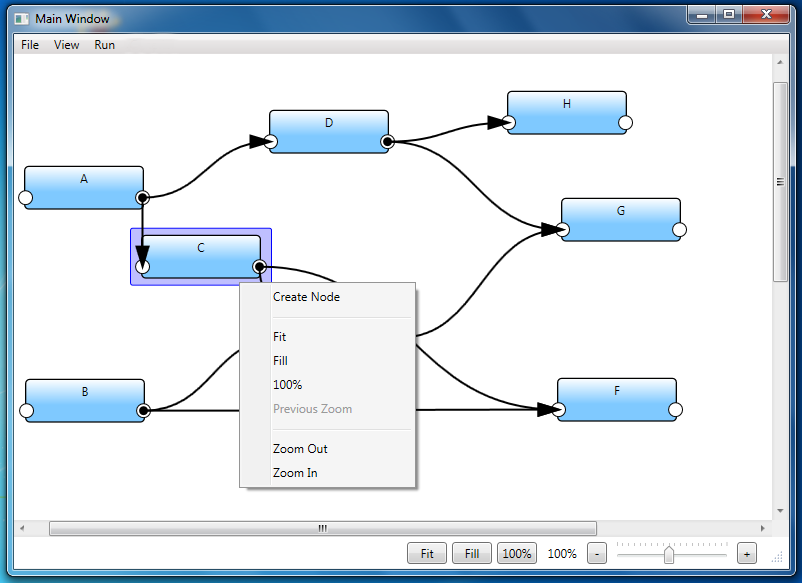
\includegraphics[scale=0.5]{app-sample-graph.png}
  \caption{Главное окно приложения} 
  \label{fig:app-sample-graph}
\end{figure}
